\section{Psychotherapy Approaches}
\label{sec:psychotherapy}

Given that our solution centers on psychotherapy approaches, we first provide a brief overview of the involved approaches in this work, which are highly representative and widely utilized in practice.

\textbf{Cognitive Behavioral Therapy (CBT)} is a structured and goal-oriented psychotherapy that empowers individuals to become their own therapists. It focuses on helping them recognize their thoughts and behaviors, providing skills to change maladaptive cognitive and behavioral patterns~\cite{Kristina2013KeyCBT}. To achieve these goals, the ABC model was developed, which suggests that ``our emotions and behaviors (C: Consequences)'' are not directly determined by life events (A: Activating Events), but rather by the way these events are cognitively processed and evaluated (B: Beliefs)''~\cite{Oltean2017AnEA}.

\textbf{Person Centered Therapy (PCT)} is a human-based therapy with the belief that the seeker is innately motivated and has the capacity for growth and self-actualization~\cite{Rogers1946SignificantAO}. It is a supportive, positive, and nondirective therapy that aims to provide seekers with a non-judgmental environment that helps them explore themselves honestly and thoroughly~\cite{Elliott2013PCT}. The therapist encourages seekers to explore their emotions and experiences in order to discover their inner strength and gain self-awareness.

\textbf{Solution-Focused Brief Therapy (SFBT)} is a competency-based model that prioritizes seekers' strengths over past failures. It facilitates the envisioning of a future where problems are resolved, constructing a pathway collaboratively with seekers. This pathway is tailored to their individual goals, resources, actions, etc.~\cite{Trepper2014SolutionFocusedTT}.

\section{Method}
\label{sec:method}

In this section, we introduce the two-step pipeline (Figure \ref{fig:prompt_resp}) of \textit{PsyMix} to fine-tune trainable LLM for better generation.
% to enhance response generation via better understanding seekers' situation with psychotherapy theories.
% \MY{just say trainable LLM here, your method is not limited to any specific model} 

\subsection{Chain-of-Psychotherapies (CoP)}
\label{sec:cot_generation}
As Section \ref{sec:intro} mentions, human counselors always analyze the seeker's situation with the perspective of various psychotherapy approaches before providing responses. However, these analyses are not explicitly manifested in dialogues. Therefore, our first step involves generating such analysis with ChatGPT, and we refer to these analyses as \textbf{\textit{Chain-of-Psychotherapies} (CoP)} (Step 1 in Figure \ref{fig:prompt_resp}).

\begin{table}[th]
    \small
    \centering
    \begin{tabular}{c|c}
    \toprule
    Psychotherapy & Perspective of Thought  \\ 
    \midrule
    CBT &  Event, Cognition, Behavior, Belief \\
    PCT &  Emotion, Self-Awareness \\
    SFBT & Goal, Resource, Exception, Action \\
    \bottomrule
    \end{tabular}
    \caption{Different Psychotherapy Thoughts}
    \label{tab:psychotherapy_thoughts}
\end{table}

We employ three widely influential psychotherapy approaches, as detailed in Section \ref{sec:psychotherapy}. To ensure the professionalism and reliability of the generated analyses, we do not allow ChatGPT to generate them independently. Instead, we collaborate with expert psychotherapists to define the specific dimensions that each psychotherapy approach should assess. These dimensions, outlined in Table \ref{tab:psychotherapy_thoughts}, represent the focal points of each approach. 
In the prompts, we instruct ChatGPT to generate analyses for every utterance made by seekers, covering all dimensions relevant to each psychotherapy approach. Detailed prompts to generate all the three CoPs are provided in Appendix \ref{apd:thought_prompt}.
% \KZ{I can't really find the prompt for ChatGPT to generate the analyses based on CBT in the figure. I also don't quite understand the difference between Response 1, 2 and naive. This figure needs to be better explained.}

\begin{figure}[th]
	\centering
	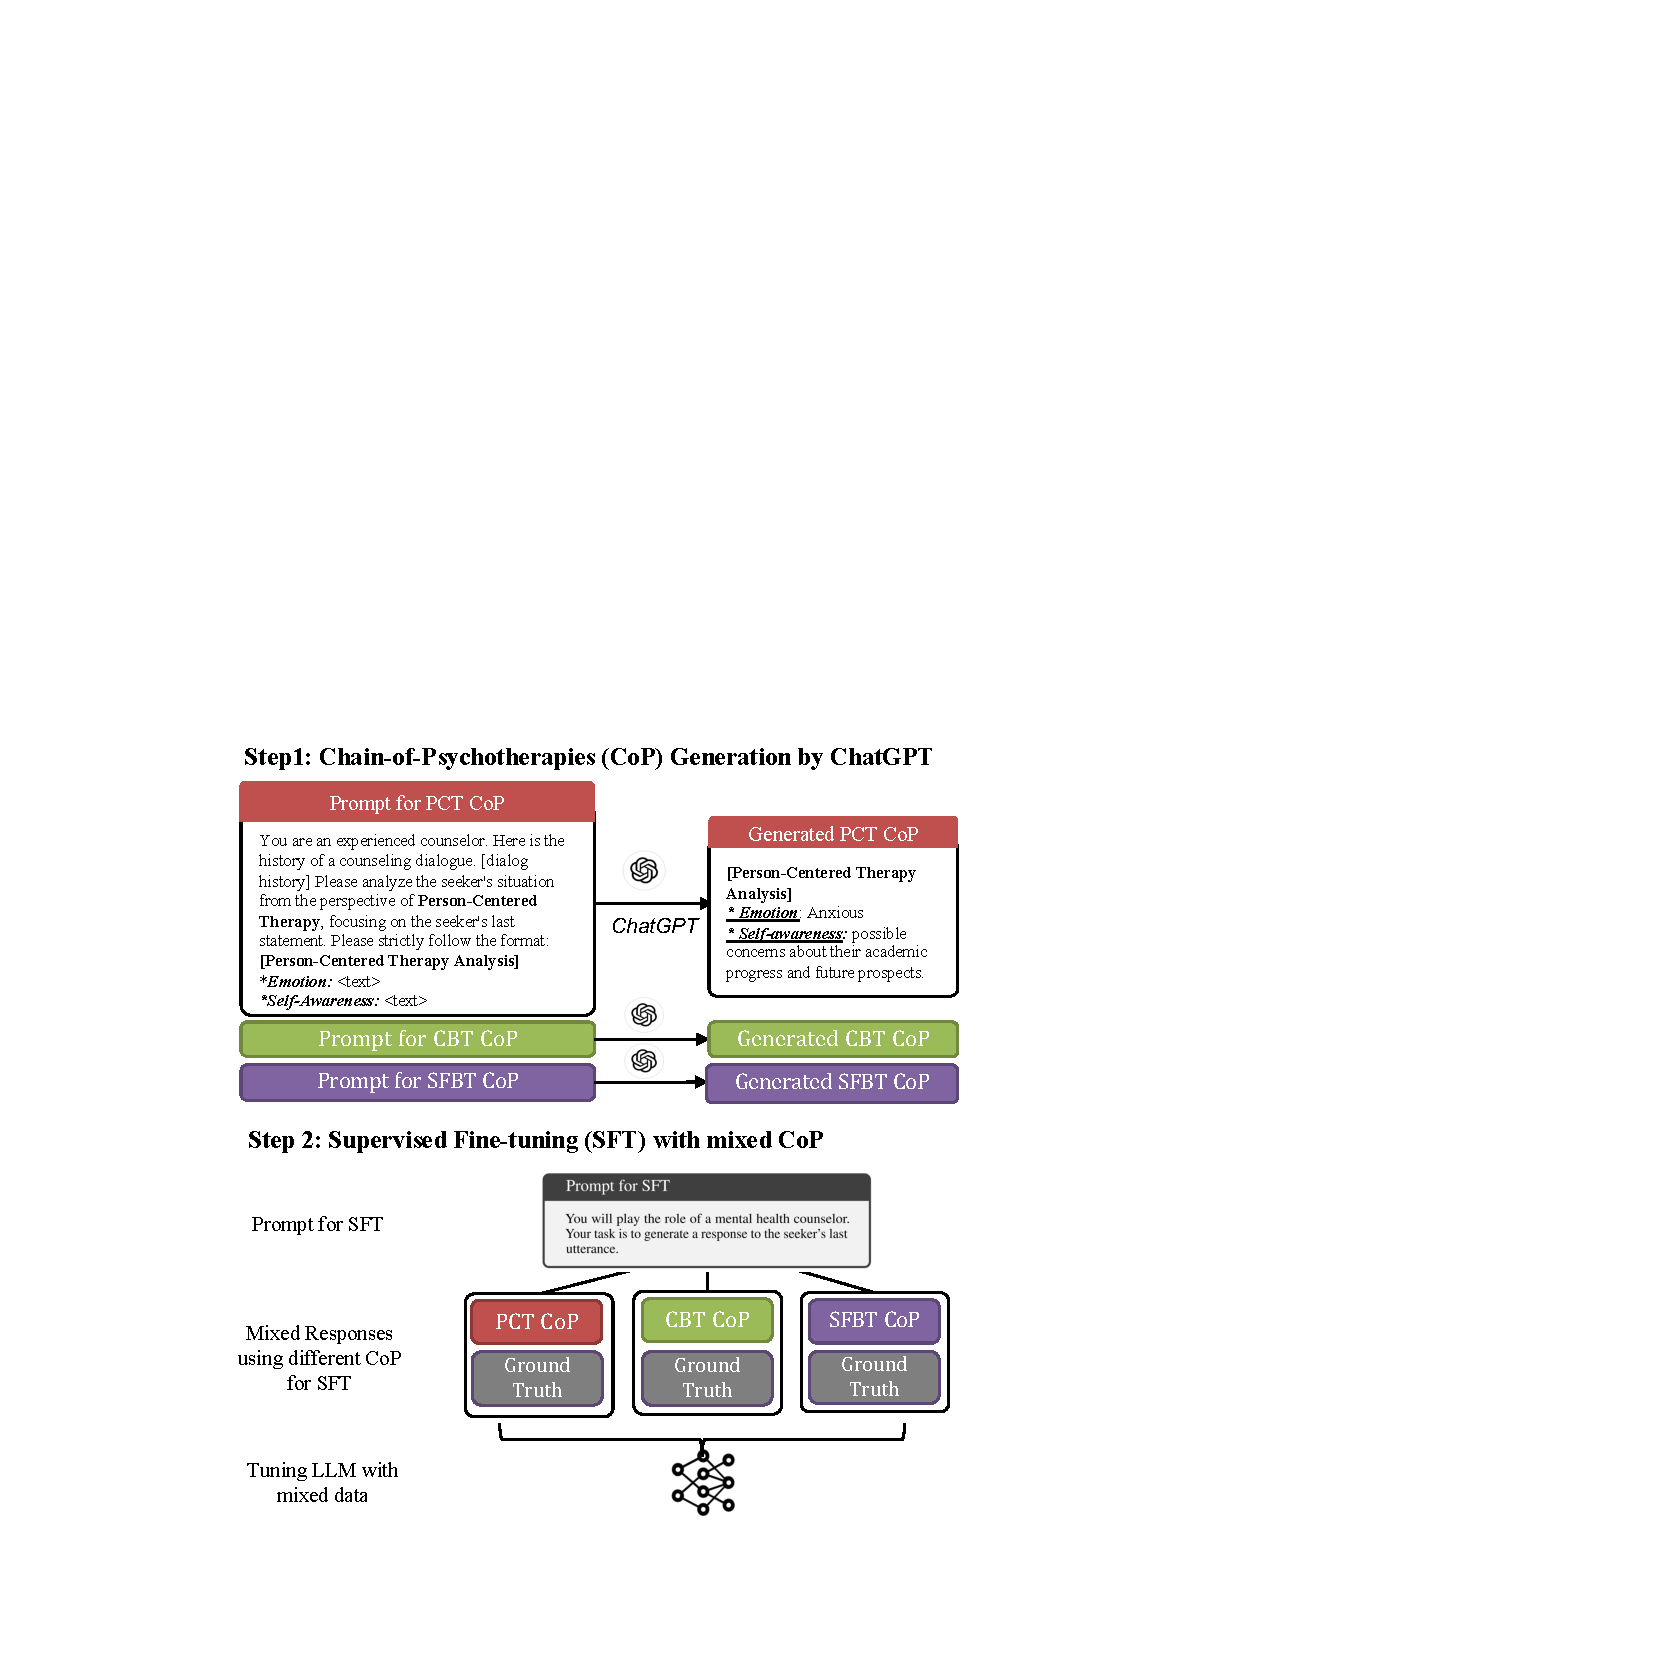
\includegraphics[width=\linewidth]{figures/prompt_resp_v2.pdf}
	\caption{Illustration of the two-step pipeline. We first generate CoPs via ChatGPT, then pack CoP with the original utterance (i.e., ground truth) in the dialog for supervised fine-tuning.}
	\label{fig:prompt_resp}
\end{figure}

% \paragraph{Generate psychotherapy thoughts via ChatGPT}
% % \KZ{I find this paragraph to be too brief. You need to say how you make ChatGPT generate those analysis to fill up the slots (Approach, analysis, respponse).} 
% Due to ChatGPT's rich knowledge in the field of psychotherapy, we leverage its capabilities to generate psychotherapy analyses for each client's utterance. To ensure the professionalism and stability of the generated  analyses, we collaborate with expert psychotherapists to establish the dimensions that each psychotherapy approach should analyze. These dimensions, as outlined in \tabref{tab:psychotherapy_thoughts}, reflect the different focal points of each psychotherapy approach on the client's state. We provide the complete prompts for generating psychotherapy thoughts in Appendix \ref{apd:thought_prompt}.

\subsection{SFT with Mixed CoP}
\label{sec:mix}
In this step, we utilize the CoP generated by ChatGPT for Supervised Fine-Tuning (SFT).
For dialog context $c$, Chain-of-Psychotherapy $p$, and the corresponding ground truth response $r$, one approach to constructing the tuning (prompt, response) pair is to set $prompt=(c, p)$ and $response = r$. However, this approach proves ineffective in inference, as in practical usage, we still need to continuously call ChatGPT's API to generate CoP. Luckily, previous study~\cite{magister-etal-2023-teaching} shows that LLMs (e.g., ChatGPT) can impart the capabilities of CoT to smaller models through knowledge distillation. Therefore, we opt to teach smaller models to generate CoP on their own, and set $prompt=c$, $response = (p, r)$, as illustrated in \figref{fig:prompt_resp}. 
% \KZ{This figure is used for two steps in the pipeline but i can't tell which is step 1 and which is step 2. I have no idea how ChatGPT generate those alternative responses.}

Moreover, inspired by the mixed thinking process in real counselling sessions, we utilize mixed Chain-of-Psychotherapies, which mixed analyses derived from all the three psychotherapy approaches for LLM-tuning. The training loss is: $L_{mix} = -\sum^3_{i=1} \log P(p_i, r| c)$,
% \begin{equation}
%     L_{mix} = -\sum^3_{i=1} \log P(p_i, r| c)
% \end{equation}
where $c$ is the context, $p_i$ is the CoP of the $i$-th psychotherapy, and $r$ is the ground truth response.
This methodology not only encourages the model to ``think'' before generating response, but also integrates strengths from various analytical perspectives. Then in inference, the model will generate $p$, where the applied psychotherapy is decided, along with $r$.
% \MY{This section now reads more like experiments part, title can be ``Mixture CoT'' and slightly tilt towards this novel setting. Method part should be about NEW things that you are proposing, in particular for a short paper}
% \KZ{I think you need to say a bit about who you did the SFT using the pairs. \secref{sec:mix} ended too suddenly.}





% In the prompt, the instructions mainly entail the task of role-playing as a mental health counselor, selecting an appropriate psychotherapy approach to analyze the seeker's state, and subsequently generating the corresponding response.

% For instance, they may initially offer unconditional positive regard in a humanistic manner to encourage seekers to express their feelings, then switch to techniques like Cognitive Behavioral Therapy (CBT)~\cite{Beck2011CognitiveBT} when addressing specific issues. 


% we fine-tune a smaller language model (Baichuan2-7B) to learn to ``think'' before generating response.


% Once the psychotherapy analyses are generated, we pack them together with the counseling dialogue context to create (prompt, response) pairs for supervised fine-tuning, as illustrated in \figref{fig:prompt_resp}. In the prompt, the instructions mainly entail the task of role-playing as a mental health counselor, selecting an appropriate psychotherapy approach to analyze the visitor's state, and subsequently generating the corresponding response. Conversely, the response includes the psychotherapy approach, the analysis based on that approach, and the reply based on the analysis.



% \begin{prompt}
% \textbf{Prompt:}
% You will play the role of a mental health counselor. Your focus should be on client-centered approach, emphasizing active listening and guidance. Utilize key communication strategies in psychotherapy such as open-ended questions, affirmation, reflective listening, and summarization. You can also draw from various psychological approaches like humanistic therapy, cognitive-behavioral therapy, and solution-focused therapy.

% As a counselor, analyze the visitor's situation based on the context of the conversation, determine which psychological approach is more suitable, and then employ the chosen approach to provide insights. Select appropriate communication strategies and generate a response to the visitor's last statement.

% Conversation context: \{context\}

% Please provide your analysis and response:

% \ \\
% \textbf{Response:}
% [Psychotherapy Approach]

% [Analysis based on psychotherapy]

% [Response based on analysis]
% \end{prompt}

% We are inspired by the observation that there are various psychotherapeutic approaches, such as Cognitive Behavioral Therapy and Humanistic Therapy. In real counseling scenarios, experienced therapists often employ a combination of these approaches during interactions with clients. For instance, they may initially offer unconditional positive regard in a humanistic manner to encourage clients to express their feelings, then switch to techniques like Cognitive Behavioral Therapy or Solution-focused Brief Therapy when addressing specific issues. By emulating this flexibility in analyzing clients' situations with multiple therapeutic perspectives, our large-scale model can better understand clients' circumstances and provide more empathetic responses.
